% Detail of the searches: in the main text for arXiv, in the online supplement for the journal.
\begin{figure*}[t]
\centering
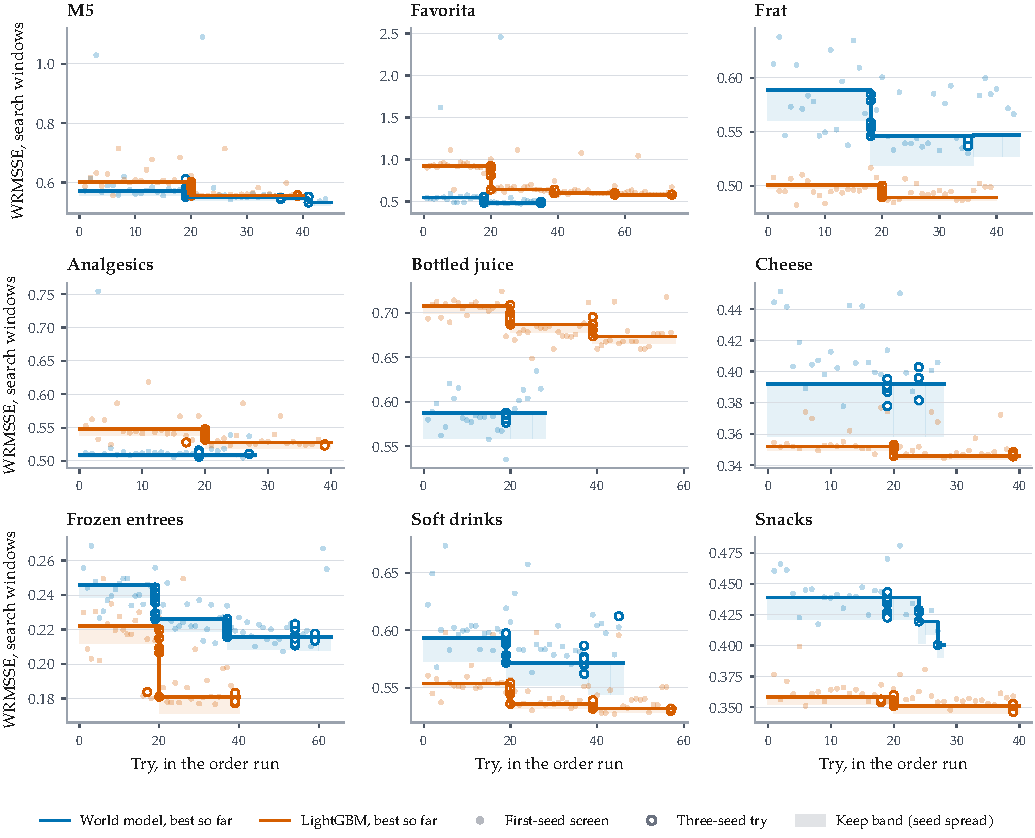
\includegraphics[width=\textwidth]{figs/fig_loop_path.pdf}
\caption{Every run of every search, in the order it was made. Faint dots are first-seed screens,
open circles are three-seed confirmations, and the step line is the best settings so far. The band
under the line is the keep bar: a change had to land below it to be kept. The world model's line
runs on into its likelihood and JEPA rounds after its own loop ends.}
\label{fig:looppath}
\end{figure*}

\subsection{What the searches kept}

The searches made \loopTries{} runs, \loopTriesWm{} of the world model and \loopTriesLgb{} of LightGBM, and kept \loopKept{} changes, \loopKeptWm{} for the world model and \loopKeptLgb{} for LightGBM.
LightGBM kept at least one change on every data set and the world model kept nothing on three of
the six Dominick's categories. No single change helped the world model everywhere
(Figure~\ref{fig:loopheat}). Weighting the loss toward high-volume series made the first seed worse on most data sets. The seven-step latent
check, kept on Favorita, was among the changes that moved Favorita most and did little elsewhere.

On the search windows the world model improved on \loopImprovedWm{} of the nine data sets and LightGBM on all
\loopImprovedLgb{} (Figure~\ref{fig:loopslopes}). The largest gain of either model was LightGBM on \loopGainLgbSet{},
from \loopGainLgbFrom{} to \loopGainLgbTo{}. The world model's largest was on \loopGainWmSet{}, from \loopGainWmFrom{} to \loopGainWmTo{}.

\begin{figure}[t]
\centering
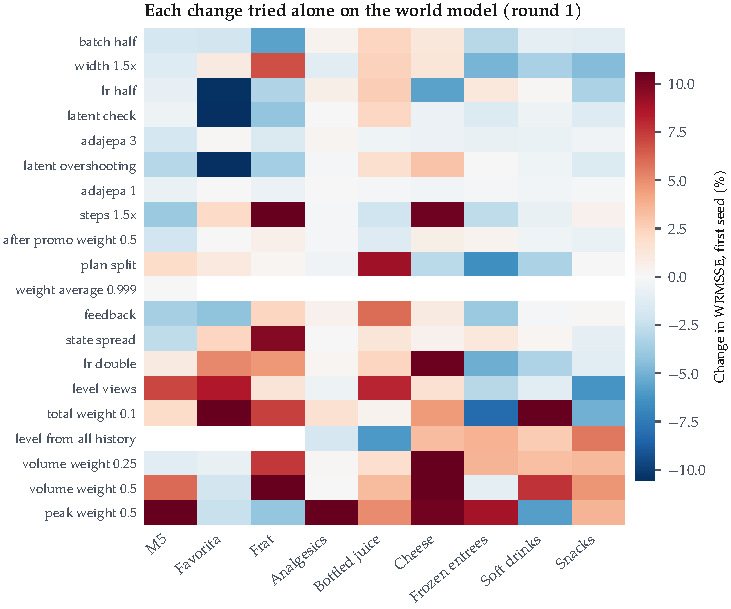
\includegraphics[width=\columnwidth]{figs/fig_loop_heat.pdf}
\caption{Each change tried alone on the world model in the first round, against that data set's
starting settings on the first seed. Blue is better. A blank cell is a change that was not on that
data set's menu.}
\label{fig:loopheat}
\end{figure}

\subsection{Did the held-out window agree?}

Only partly. Across every three-seed run, the change on the search windows and the change on the
held-out window are correlated at \loopHeldCorrWm{} for the world model and \loopHeldCorrLgb{} for LightGBM
(Figure~\ref{fig:loopheldout}). A change that helps on the search windows is a weak guide to the
next window. The world model's final settings were worse than its starting settings on the
held-out window on \loopHeldWorseWm{} data sets, most on \loopHeldWorstWmSet{} (\loopHeldWorstWmFrom{} to \loopHeldWorstWmTo{}), and
LightGBM's on \loopHeldWorseLgb{}, most on \loopHeldWorstLgbSet{} (\loopHeldWorstLgbFrom{} to \loopHeldWorstLgbTo{}). This is why the paper reports the final settings on windows that the
searches never saw, in Section~\ref{sec:results}, and not the search scores.

\begin{figure}[t]
\centering
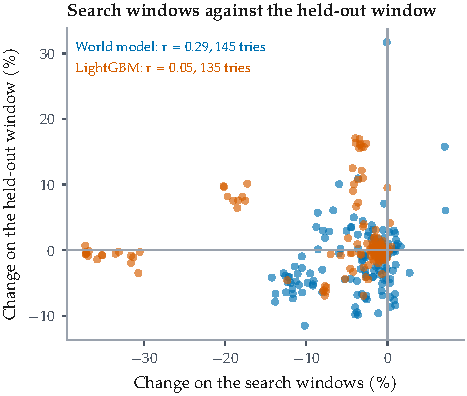
\includegraphics[width=\columnwidth]{figs/fig_loop_heldout.pdf}
\caption{Each three-seed run's change on the search windows against its change on the held-out
window, both against the starting settings of its search.}
\label{fig:loopheldout}
\end{figure}

\subsection{Seed noise, one copy against five}
\label{sec:loopnoise}

A single world-model fit is noisy enough to hide most of the changes the loop tries. On the six
Dominick's categories the three seeds of the starting settings differ from their mean by a
standard deviation of \loopSeedSdOne\% for a single fit and \loopSeedSdFive\% for a five-copy average
(Figure~\ref{fig:loopnoise}). The
single-fit search on cheese had a bar of \loopOneCheBar{} and kept nothing; with the average the bars on the
Dominick's categories were between \loopBarLoWm{} and \loopBarHiWm{}. LightGBM's seeds differ much less, and its
bars were between \loopBarLoLgb{} and \loopBarHiLgb{}.

\begin{figure}[t]
\centering
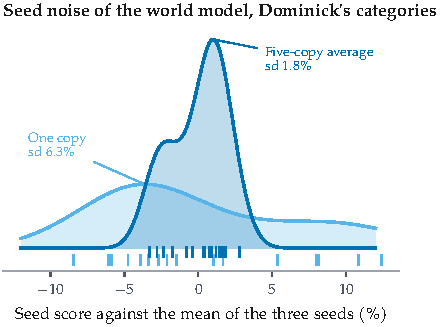
\includegraphics[width=\columnwidth]{figs/fig_loop_noise.pdf}
\caption{The starting settings' three seed scores on each Dominick's category, as a share of their
mean, for a single world-model fit and for the five-copy average. Ticks are the scores.}
\label{fig:loopnoise}
\end{figure}

\begin{figure*}[t]
\centering
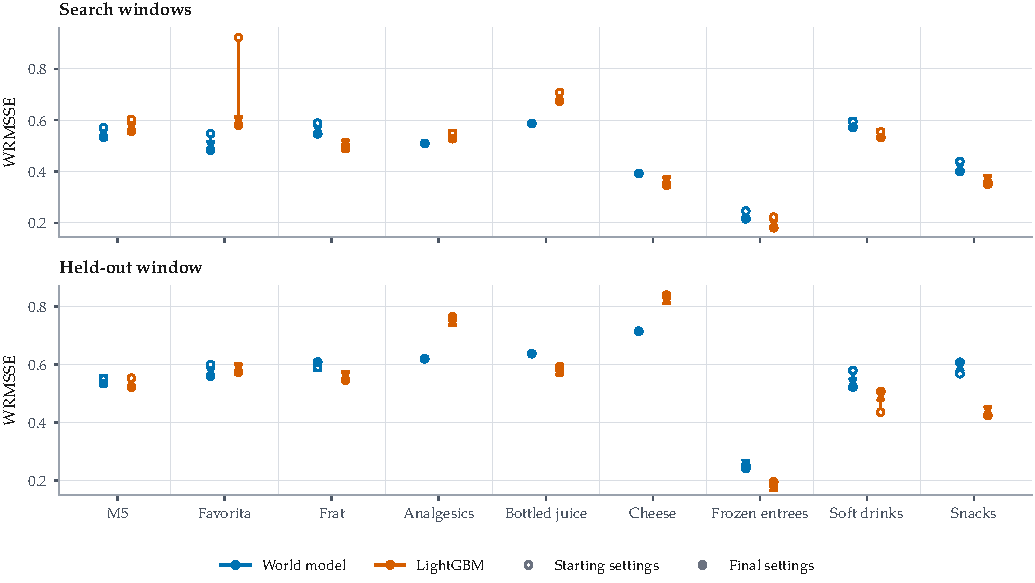
\includegraphics[width=\textwidth]{figs/fig_loop_slopes.pdf}
\caption{Each model's starting and final settings on each data set. Open circles are the starting
settings and filled circles the final settings, on the search windows (top) and the held-out
window (bottom).}
\label{fig:loopslopes}
\end{figure*}
